\documentclass[12pt,a4paper]{article}

% Language and typography
\usepackage[american]{babel}
\usepackage[T1]{fontenc}
\usepackage{lmodern}
\usepackage{microtype}
\usepackage{csquotes}

% Page layout
\usepackage[margin=2.5cm]{geometry}
\usepackage{parskip}

% Figures, tables, and mathematics
\usepackage{algorithm}
\usepackage{algpseudocode}
\usepackage{graphicx}
\usepackage{booktabs}
\usepackage{threeparttable}
\usepackage{amsmath}
\usepackage{float}

% APA 7 citations (requires Biber)
\usepackage[
    style=ieee,
    backend=biber
]{biblatex}
\addbibresource{references.bib}

% Paper metadata
\title{\textbf{ACIT 4610 -- Final Group Project}}

\author{
    Alexander Hoem \and
    Michael Huse \and
    Noah \O fsti \and
    Niklas Goldhan
}

\date{\today}

\begin{document}

% Title page
\begin{titlepage}
    \centering

    \vspace*{3cm}

    {\LARGE\bfseries
    ACIT 4610 -- Final Group Project
    \par}

    \vspace{2cm}

    {\Large Group 1} \\
    {\large
    Alexander Hoem\\
    Michael Huse\\
    Noah \O fsti\\
    Niklas Goldhan
    \par}

    \vspace{1.5cm}

    Department of Computer Science\\
    Oslo Metropolitan University

    \vspace{1cm}

    ACIT4610: Evolutionary Artificial Intelligence and Robotics
    

    \vspace{1cm}

    Professor: Kazi Shah Nawaz Ripon

    \vfill

    \today

\end{titlepage}

% Main content
\section{Bees Algorithm}
The bees algorithm is a swarm intelligence algorithm which mimics the food foraging behavior of bees. It was introduced by Pham and colleagues in 2006 \cite{Pham2006}. It has applications in both combinatorial and functional optimization.

% \begin{figure}[H]
%     \centering
%     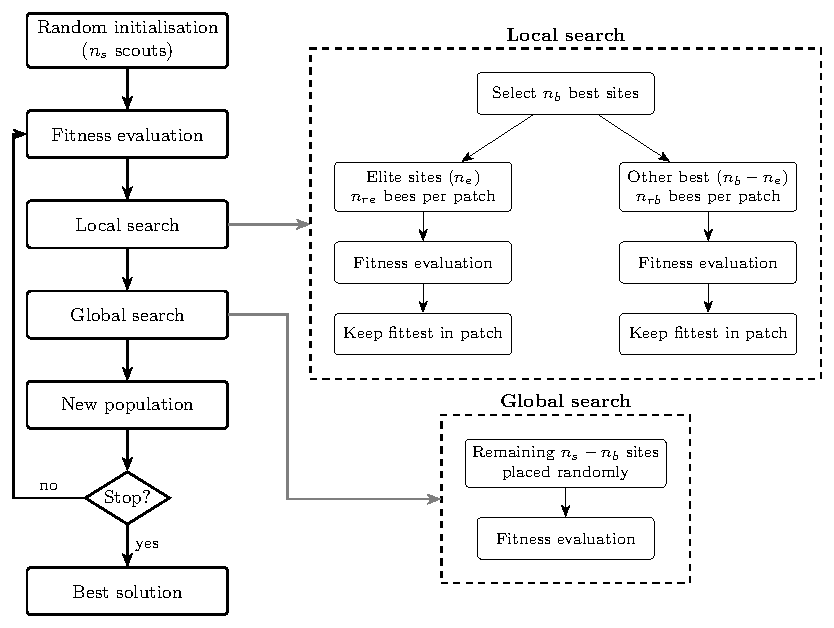
\includegraphics[width=0.9\linewidth]{assets/bees_flowchart.pdf}
%     \caption{Flowchart of the Bees Algorithm. Adapted from Pham's 2009 paper\cite{Pham2009}.}
%     \label{fig:bees-flowchart}
% \end{figure}

% !TEX root = ../main.tex
\subsection{Continuous Function Optimization}
In this section, the Bees Algorithm is applied for the purposes of continuous function optimization.
Here the representation is a vector of D real numbers, where D is the number of dimensions.

The functions we aim to optimize are unshifted, noiseless functions from Surjanovic and Bingham's Simon Fraser University collection \cite{surjanovic_bingham}. 

\textbf{Sphere:} 

\begin{equation}
    f(x)=\sum_{i=1}^{D}x_i^2
\end{equation}
Bounds: \(x_i \in [-5.12,5.12]\). Checked: \(f(0)=0\) and \(f(1) = D\).

\textbf{Rosenbrock:}

\begin{equation}
    f(x)=\sum_{i=1}^{D-1}[100(x_{i+1}-x_i^2)^2+(1-x_i)^2]
\end{equation}
Bounds: \(x_i \in [-5,10]\). Checked: \(f(1)=0\) and \(f(0)=D-1\).

\textbf{Rastrigin:}
\begin{equation}
    f(x)=10D+\sum_{i=1}^{D}[x_i^2-10cos(2\pi x_i)]
\end{equation}
Bounds: \(x_i \in [-5.12,5.12]\). Checked: \(f(0)=0\) and \(f(0.5)=20.25D\).

\textbf{Ackley:}
\begin{equation}
    f(\mathbf{x}) = -20 \exp\left(-0.2 \sqrt{\frac{1}{D} \sum_{i=1}^{D} x_i^2}\right) - \exp\left(\frac{1}{D} \sum_{i=1}^{D} \cos(2\pi x_i)\right) + 20 + e
\end{equation}
Bounds: \(x_i \in [-32.768,32.768]\). Checked: \(f(0)=0\) and \(f(1) \approx 3.62538\).

The numpy function implementations were tested with a floating-point tolerance of $10^{-12}$ to confirm the global minimum along with one other control point derived from the function equations. This was done in "\textit{check\_functions.py}", with all checks passing.

\vfill

\subsubsection{Implementation}
This implementation of the Bees Algorithm is primarily based upon the implementation described in the 2009 paper from Pham \& Castellani \cite{Pham2009}. In contrast to the TSP problem, the scout bees are initialized uniformally within the function bounds, and ranked with an ascending sort.

\begin{table}[H]
\centering
\caption{Parameters and values used in the experiment}
\label{tab:bees-params}
\begin{tabular}{lll}
\hline
\textbf{Symbol} & \textbf{Value} & \textbf{Description} \\
\hline
$n_s$        & 13     & Number of scout bees (sites) \\
$n_b$        & 6      & Number of best sites  \\
$n_e$        & 3      & Number of elite sites among $n_b$ \\
$n_{re}$     & 9      & Bees recruited per elite site \\
$n_{rb}$     & 6      & Bees recruited per remaining best site \\
$ngh$        & 0.1    & Initial neighborhood size as fraction of bounds \\
$stlim$      & 20     & Stagnant cycles before a site is abandoned \\
$\alpha$     & 0.95   & Neighborhood shrink factor ($0 < \alpha < 1$) \\
$E_{\max}$   & 30,000 & Maximum number of function evaluations \\
\hline
\end{tabular}
\end{table}

\begin{algorithm}[H]
\caption{Bees Algorithm with Site Abandonment}
\label{alg:beesfunc}
\begin{algorithmic}[1]
\State Initialize and evaluate $n_s$ random sites within bounds
\While{fewer than $E_{\max}$ evaluations}
    \State Rank sites by fitness (ascending)
    \For{each of the $n_b$ best sites}
        \State Search neighborhood with $n_{re}$ bees if elite, else $n_{rb}$
        \If{a better solution is found}
            \State Move site there and reset stagnation counter
        \Else
            \State Shrink neighborhood by $\alpha$ and increment counter
            \If{counter $\geq stlim$}
                \State Abandon site and reinitialize randomly
            \EndIf
        \EndIf
    \EndFor
    \State Reinitialize remaining $n_s - n_b$ sites randomly
\EndWhile
\State \Return best solution found $(\mathbf{x}^*, f(x^*))$
\end{algorithmic}
\end{algorithm}

The main difference from the original 2006 implementation is the introduction of site abandonment.
This addition allows for more exploration in the problem space by abandoning sites that have not improved for the last $stlim$ cycles.
A given neighborhood is clipped to the bounds of the problem space, and neighborhood shrinkage makes up for the large initial range, honing in on promising areas.
Since running the full benchmark was quite fast with the cap of 30,000 evaluations, it was feasible to do a sweep to find general parameters that achieve good scores overall on this varied set of problems.
The only constant was $ngh=0.1$, as it was specified in the assignment brief.

\subsubsection{Results}

Each function was run 10 times at $D=10$ and $D=30$ with a budget of 30,000 evaluations per run.
The settings in Table~\ref{tab:bees-params} were used along with per-run seeds derived from a single master seed, 42.

\begin{table}[ht]
\centering
\caption{Final objective values over 10 runs (30,000 evaluations each).}
\label{tab:bafuncsummary}
\begin{tabular}{llrrrrr}
\toprule
Function & $D$ & Mean initial & Best & Mean & Std & Runtime (s) \\
\midrule
Sphere     & 10 & 46.2 & $2.44\times10^{-19}$ & $5.38\times10^{-19}$ & $1.90\times10^{-19}$ & 0.090 \\
           & 30 & 189.1 & $2.33\times10^{-12}$ & $1.19\times10^{-11}$ & $8.07\times10^{-12}$ & 0.094 \\
Rosenbrock & 10 & $3.04\times10^{5}$ & 0.0434 & 3.06 & 2.02 & 0.171 \\
           & 30 & $2.23\times10^{6}$ & 20.1 & 25.2 & 2.31 & 0.175 \\
Rastrigin  & 10 & 134.8 & 20.9 & 24.6 & 3.03 & 0.146 \\
           & 30 & 462.9 & 88.6 & 133.4 & 25.0 & 0.153 \\
Ackley     & 10 & 20.5 & $4.51\times10^{-9}$ & $9.72\times10^{-9}$ & $3.99\times10^{-9}$ & 0.169 \\
           & 30 & 20.9 & 1.16 & 2.03 & 0.499 & 0.175 \\
\bottomrule
\end{tabular}
\end{table}

Table~\ref{tab:bafuncsummary} summarises the results of all four functions, and Figure~\ref{fig:ba-boxplots} shows the distribution of final values at $D=30$.
The algorithm performs best on Sphere, reaching the global minimum of 0 to within $10^{-11}$. 
Ackley is also solved at $D=10$, but at $D=30$ runs land in local minima. 
On Rosenbrock the algorithm makes good progress at $D=10$, falling from a mean of $10^5$ to $3.06$, but ultimately does not reach global optimum. 
Performance is the worst on Rastrigin, with mean final values of 24.6 and 133.4 respectively.

\begin{figure}[H]
    \centering
    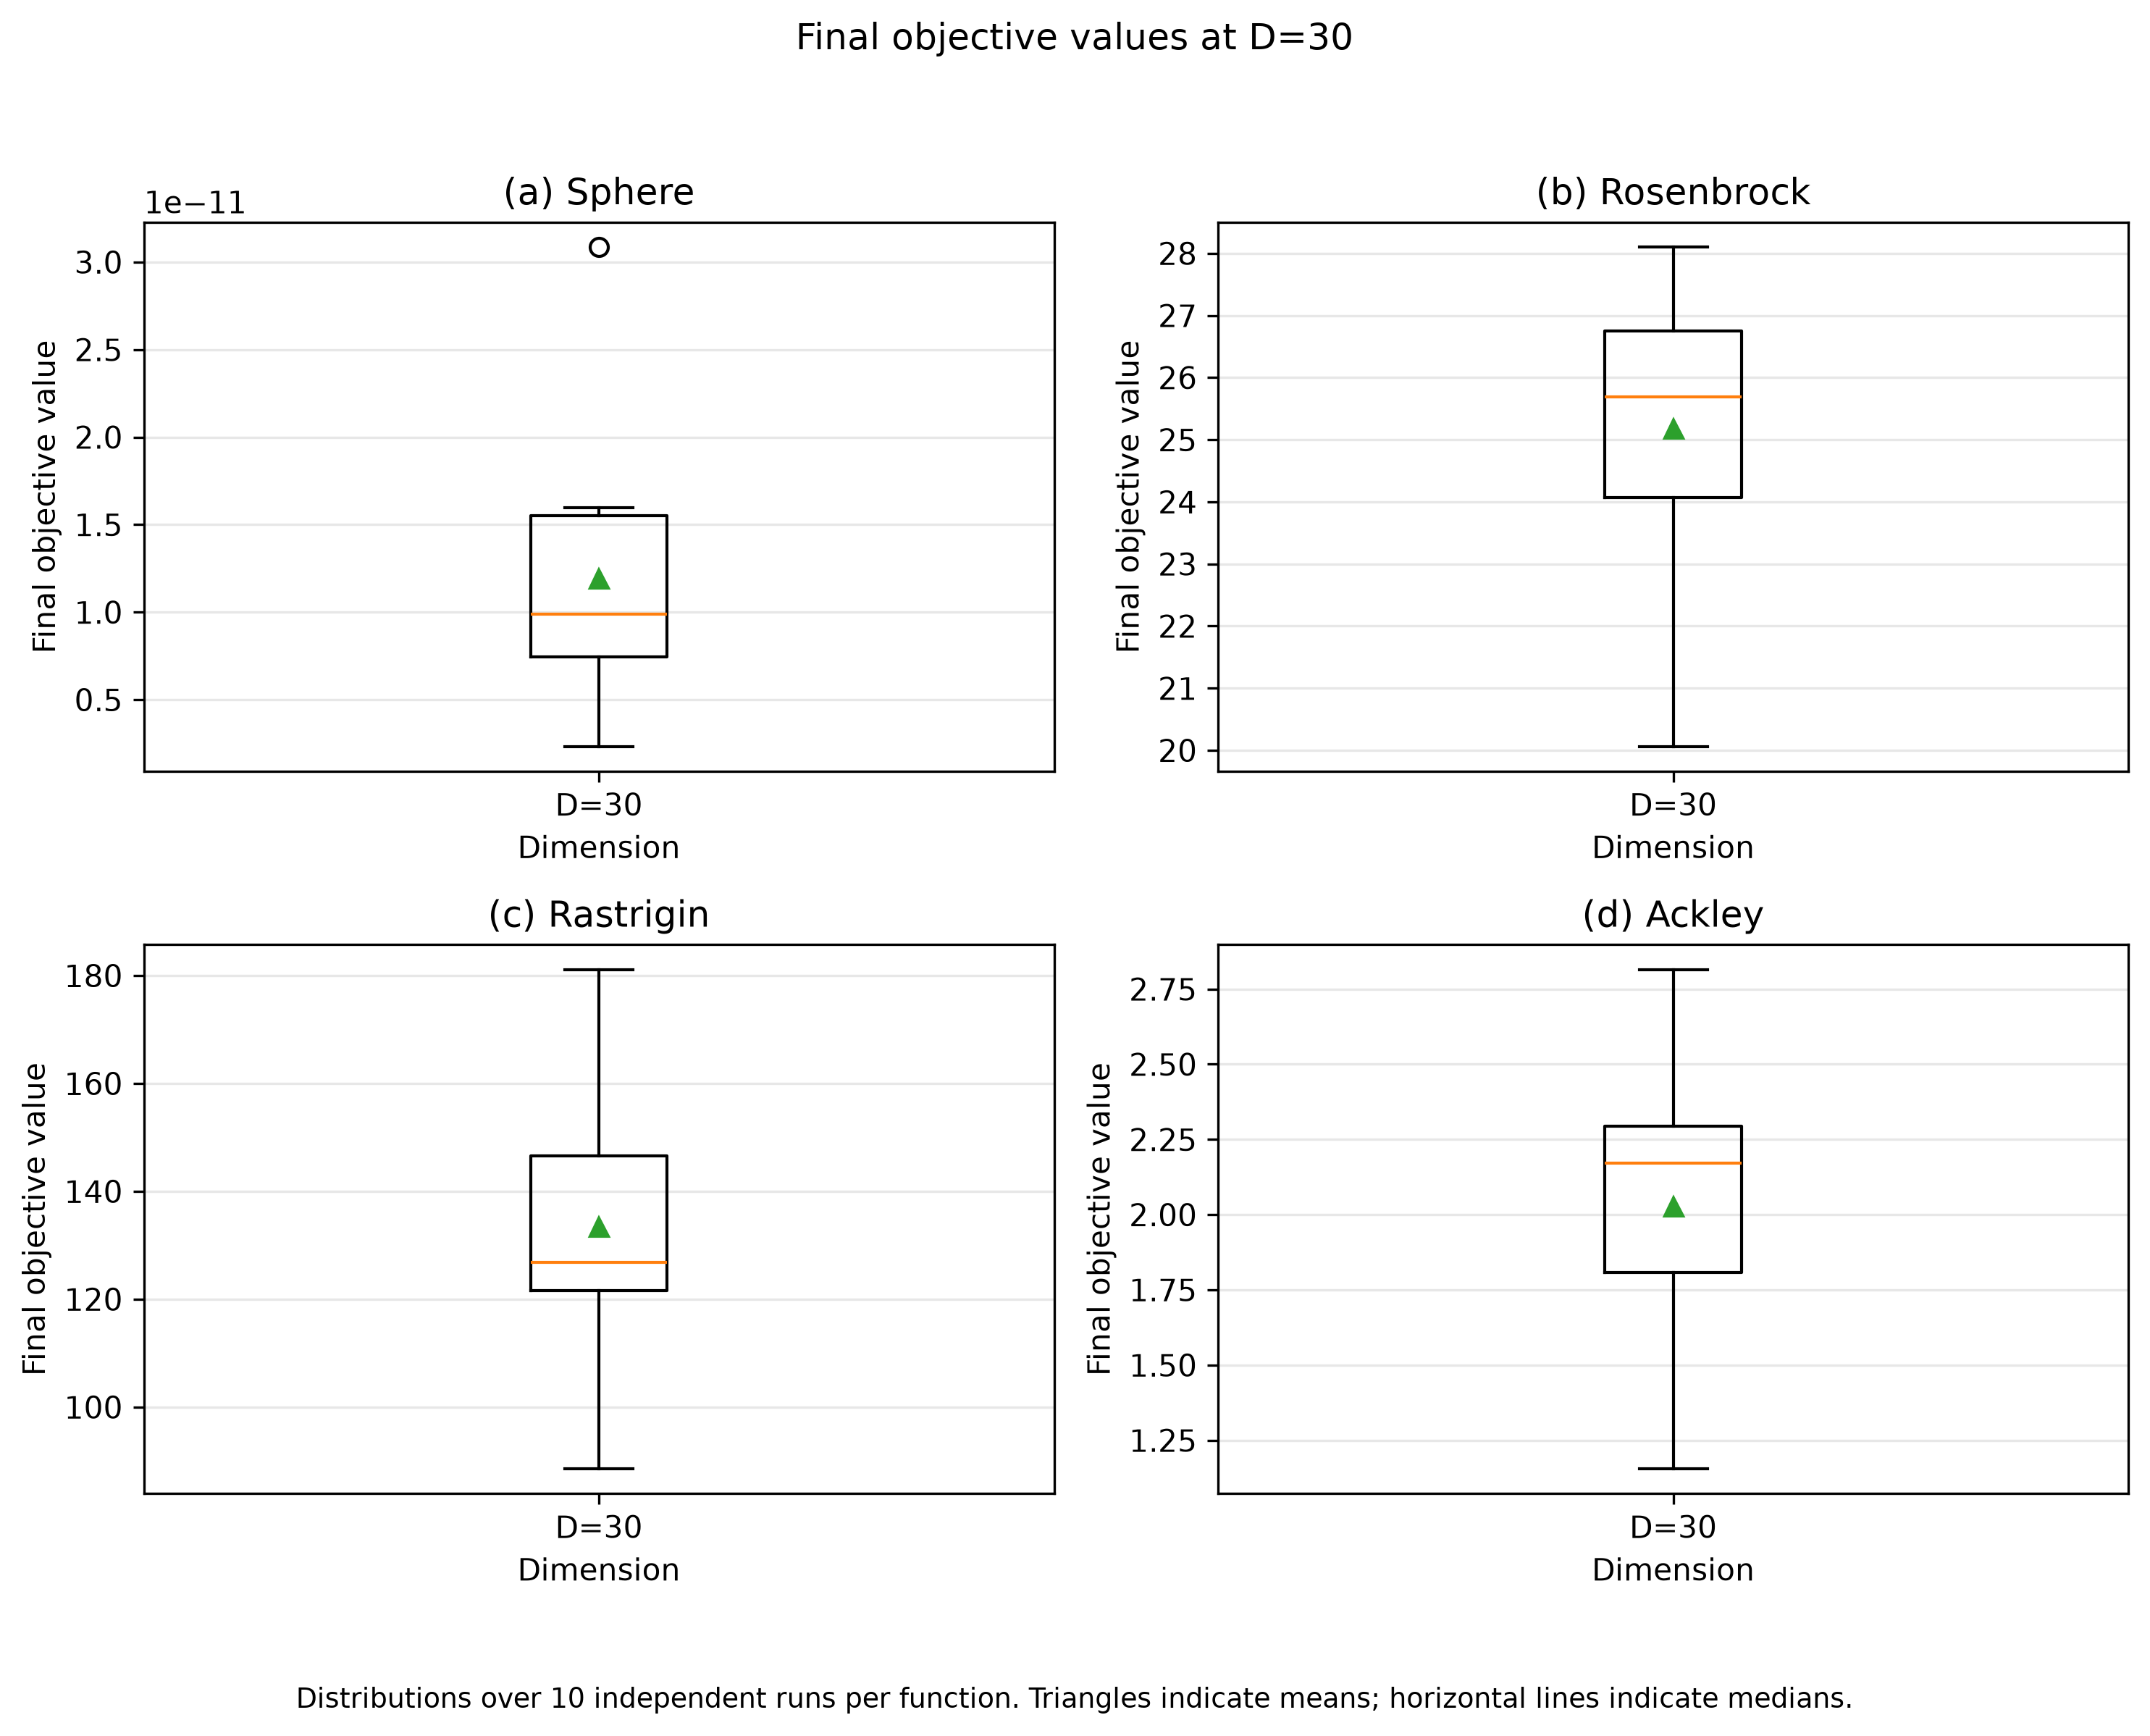
\includegraphics[width=0.8\linewidth]{results/final_boxplots_d30.png}
    \caption{Boxplots of final objectives for all four functions at D=30.}
    \label{fig:ba-boxplots}
\end{figure}

\subsection{Discussion}

To understand the implementation's shortcomings, an examination of the worst case is in order.
Figure~\ref{fig:ba-rastrigin} shows how the algorithm quickly converges before stalling at $\approx$5,000 evaluations. 
This highlights the main issue with the local search

\begin{figure}[H]
    \centering
    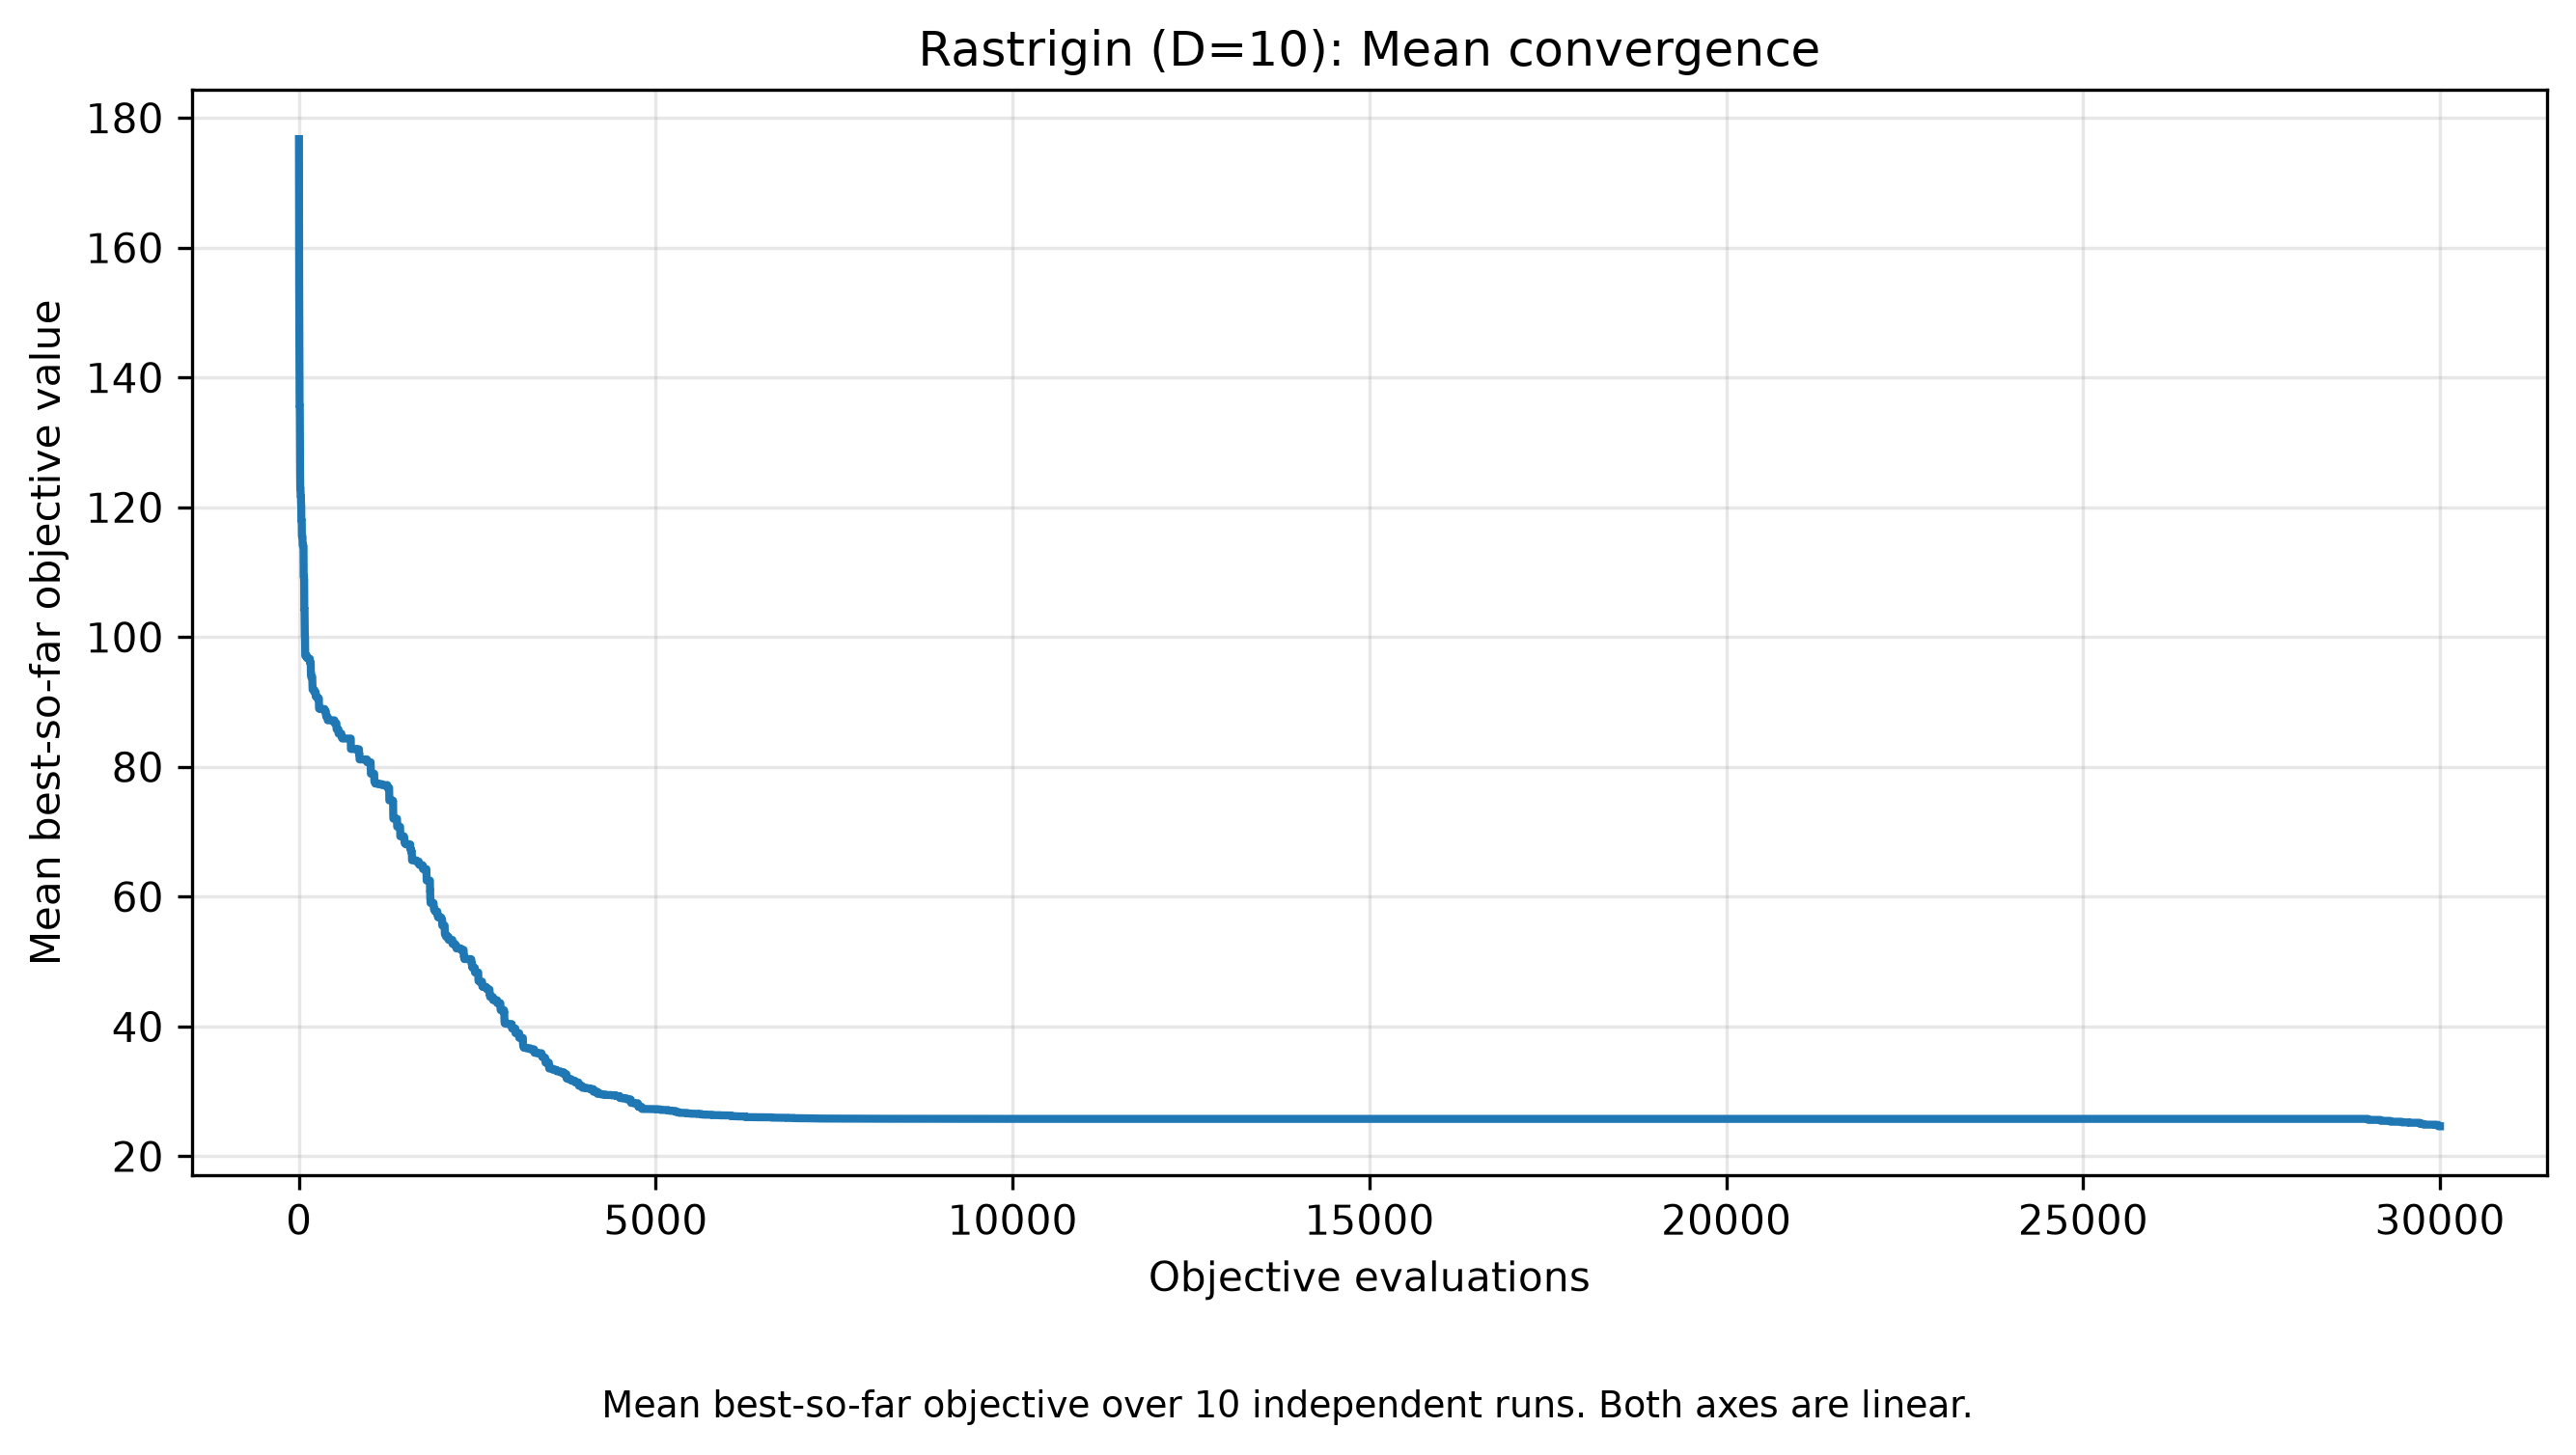
\includegraphics[width=0.8\linewidth]{results/rastrigin_convergence.png}
    \caption{Rastrigin D=10: evaluations against mean best-so-far objective across 10 runs.}
    \label{fig:ba-rastrigin}
\end{figure}

% !TEX root = ../main.tex

\newpage
% \section{Problem 1: Bees Algorithm}
% The Bees Algorithm (BA) is a population-based search algorithm inspired by how honey bees forage for food.
% In nature, scout bees search randomly for good flower patches and use a waggle dance at the hive to recruit follower bees based on the quality of each patch.
% The algorithm uses this same idea to balance global exploration across the whole search space with focused local exploitation around the best solutions found so far.
% In this problem, the Basic BA (without neighbourhood shrinking or site abandonment) is applied to both a discrete route-planning task in Part~A and continuous function optimization in Part~B.

\subsection{Part A: Travelling Salesman Problem (TSP)}

\subsubsection{Problem and Data}
The Travelling Salesman Problem (TSP) models a delivery vehicle that starts at a depot, visits \(n\) distinct cities exactly once and returns to the starting depot.
Because the distance between any two cities is the same in both directions, this is a symmetric TSP.
The goal is to find the shortest complete round trip.

Each candidate route is stored as an ordered list of city numbers, \(\pi = (\pi_1, \pi_2, \dots, \pi_n)\).
City~1 is always fixed at the first position (\(\pi_1 = 1\)) so that every route starts at the same depot and duplicate shifted versions of the same loop are avoided.
City~1 is only added to the end of the route when calculating the return distance or plotting the closed loop.
The total length \(L(\pi)\) of a route is the sum of the distances between consecutive cities plus the return trip from the last city back to City~1:
\begin{equation}
    L(\pi) = \sum_{i=1}^{n-1} d_{\pi_i, \pi_{i+1}} + d_{\pi_n, \pi_1}.
\end{equation}
To check how close a possible route is to the known best solution \(L^*\), a percentage gap is calculated as:
\begin{equation}
    \text{Gap}(\%) = 100 \times \frac{L_{\text{BA}} - L^*}{L^*}.
\end{equation}

The experiments test six standard 2D symmetric benchmark instances from the TSPLIB library.
Table~\ref{tab:benchmark_instances} lists the exact filenames, city counts, distance types and known optimal route lengths.
These optimal lengths are only used at the end to check solution quality and compute percentage gaps, never to initialize or guide the search.

\begin{table}[htbp]
\caption{TSPLIB 2D Symmetric Benchmark Instances}
\label{tab:benchmark_instances}
\begin{threeparttable}
\begin{tabular}{llclr}
\toprule
Instance & Filename & Cities (\(n\)) & Edge Weight Type & Known Optimum (\(L^*\)) \\
\midrule
\texttt{eil51}    & \texttt{eil51.tsp}    & 51  & \texttt{EUC\_2D} & 426 \\
\texttt{berlin52} & \texttt{berlin52.tsp} & 52  & \texttt{EUC\_2D} & 7,542 \\
\texttt{st70}     & \texttt{st70.tsp}     & 70  & \texttt{EUC\_2D} & 675 \\
\texttt{eil76}    & \texttt{eil76.tsp}    & 76  & \texttt{EUC\_2D} & 538 \\
\texttt{kroA100}  & \texttt{kroA100.tsp}  & 100 & \texttt{EUC\_2D} & 21,282 \\
\texttt{ch150}    & \texttt{ch150.tsp}    & 150 & \texttt{EUC\_2D} & 6,528 \\
\bottomrule
\end{tabular}
\begin{tablenotes}[flushleft]
\small
\item \textit{Note.} All instances use 2D Euclidean rounded distances. Known optimum values (\(L^*\)) are taken from TSPLIB reference documentation.
\end{tablenotes}
\end{threeparttable}
\end{table}

Following the TSPLIB \texttt{EUC\_2D} rule, the distance \(d_{ij}\) between two cities at coordinates \((a_i, b_i)\) and \((a_j, b_j)\) is calculated by adding \(0.5\) to the Euclidean distance and rounding downward to the nearest integer:
\begin{equation}
    d_{ij} = \left\lfloor \sqrt{(a_i - a_j)^2 + (b_i - b_j)^2} + 0.5 \right\rfloor.
\end{equation}
Each individual part of the route is rounded before summing the full route, including the return leg.
At the start of each experiment, all distances are stored in an \(n \times n\) distance table, so that route lengths can be read quickly during the search.

Before running the algorithm, the data loader runs several validation checks on each input file.
It verifies that the required headers (\texttt{NAME}, \texttt{TYPE}, \texttt{DIMENSION}, \texttt{EDGE\_WEIGHT\_TYPE} and \texttt{NODE\_COORD\_SECTION}) are present and confirms that \texttt{TYPE} is \texttt{TSP} and \texttt{EDGE\_WEIGHT\_TYPE} is \texttt{EUC\_2D}.
It also checks that \texttt{DIMENSION} matches the exact number of coordinate rows read from the file and that all city identifiers are unique.
After each run, the returned best route is checked to confirm that City~1 is at the start and every city appears exactly once.

\subsubsection{Implementation and Experimental Setup}
To explore nearby routes around a selected site, two neighborhood operators are implemented and compared.
Both operators leave City~1 fixed at the first position and pick two random positions from the remaining cities \(\{2, \dots, n\}\).
Each recruited forager bee creates one neighbor by applying a single random move, because both moves only rearrange existing cities, every new route remains a valid permutation automatically without needing any repair step or bounds handling.

The \textit{swap operator} picks two different positions \(i\) and \(j\) that are not City~1 and exchanges the cities at those two spots.
If the two chosen positions are not right next to each other, swapping them breaks up to four existing connections in the route and forms new ones.
The \textit{segment reversal operator} also picks two different positions \(i < j\) that are not City~1, but instead reverses the order of the entire segment of cities between them.
Reversing a segment breaks only two connections at the ends of the segment while keeping all city connections inside the segment intact in reverse order.

The Basic BA begins by creating an initial population of \(n = 20\) scout bees with random routes, keeping City~1 fixed as the start.
Each scout route is evaluated for its total length, the initial best value is recorded and the population is sorted from shortest to longest route.
In every search cycle, the algorithm performs local search on the \(m = 6\) best routes.
The top \(e = 2\) elite routes each recruit \(n_e = 20\) forager bees, while the remaining \(m - e = 4\) selected routes each recruit \(n_s = 8\) forager bees.
Within each flower patch, every recruited forager tests one mutated neighbor around the site's route and only the single shortest route found in that patch is kept for the next population.
To keep exploring new regions of the search space, the remaining \(n - m = 14\) bees are sent out as fresh random scouts (global search).
At the end of the cycle, the 20 new bees (2 elite patch winners, 4 non-elite patch winners and 14 fresh random scouts) replace the old population and are sorted again by shortest route length.

Each full cycle performs \((2 \times 20) + (4 \times 8) + 14 = 86\) objective evaluations.
Every run has a strict budget of 30,000 objective evaluations, which counts the initial scouts, all recruited neighbors (even when they are worse and not kept) and all fresh random scouts.
The loop stops immediately once 30,000 evaluations are reached, allowing an incomplete final cycle and records the full best-so-far history along with the final best route.
All implementation details and parameter settings are also documented in the project \texttt{README.md}.

To compare the two neighborhood operators fairly, both are tested using the exact same BA settings and the same 10 independent random seeds (\(1, 2, 4, 8, 16, 32, 64, 128, 256, 512\)).
Across the six TSPLIB instances and two operators, this gives 120 runs in total.
For each case, the experiments record the best route length, mean route length, standard deviation (\(SD\)), mean percentage gap and mean runtime in seconds.

\subsubsection{Results}
Table~\ref{tab:summary_statistics} summarizes the performance of both operators across all six benchmark instances over the 10 runs.
On every instance, segment reversal achieves much shorter routes, lower mean gaps and lower standard deviations than the swap operator, while taking almost the same runtime (between 0.08~s and 0.28~s per run).
For the two smallest instances (\texttt{eil51} and \texttt{berlin52}), segment reversal reaches mean gaps of 7.35\% and 7.93\%, compared to 33.24\% and 37.32\% for swap.

\begin{table}[H]
\caption{Performance Comparison of Swap and Segment Reversal Operators on TSPLIB Instances}
\label{tab:summary_statistics}
\begin{threeparttable}
\small
\setlength{\tabcolsep}{4pt}
\begin{tabular}{lclrccccc}
\toprule
Instance & Cities & Operator & \shortstack[c]{Optimum\\(\(L^*\))} & Best & Mean & \(SD\) & \shortstack[c]{Mean\\Gap (\%)} & \shortstack[c]{Mean\\Runtime (s)} \\
\midrule
\texttt{eil51} & 51 & Swap & 426 & 535 & 567.6 & 20.16 & 33.24\% & 0.08 \\
 & 51 & \textbf{Reversal} & 426 & \textbf{444} & \textbf{457.3} & \textbf{9.97} & \textbf{7.35\%} & 0.09 \\
\addlinespace
\texttt{berlin52} & 52 & Swap & 7,542 & 9,455 & 10,356.8 & 501.44 & 37.32\% & 0.11 \\
 & 52 & \textbf{Reversal} & 7,542 & \textbf{7,874} & \textbf{8,140.0} & \textbf{208.44} & \textbf{7.93\%} & 0.12 \\
\addlinespace
\texttt{st70} & 70 & Swap & 675 & 1,026 & 1,156.0 & 64.53 & 71.26\% & 0.13 \\
 & 70 & \textbf{Reversal} & 675 & \textbf{710} & \textbf{761.9} & \textbf{21.09} & \textbf{12.87\%} & 0.14 \\
\addlinespace
\texttt{eil76} & 76 & Swap & 538 & 755 & 823.8 & 37.39 & 53.12\% & 0.14 \\
 & 76 & \textbf{Reversal} & 538 & \textbf{599} & \textbf{616.7} & \textbf{13.00} & \textbf{14.63\%} & 0.14 \\
\addlinespace
\texttt{kroA100} & 100 & Swap & 21,282 & 48,629 & 50,602.9 & 1,143.43 & 137.77\% & 0.19 \\
 & 100 & \textbf{Reversal} & 21,282 & \textbf{29,047} & \textbf{30,208.7} & \textbf{1,005.21} & \textbf{41.94\%} & 0.21 \\
\addlinespace
\texttt{ch150} & 150 & Swap & 6,528 & 15,920 & 18,565.4 & 1,073.31 & 184.40\% & 0.27 \\
 & 150 & \textbf{Reversal} & 6,528 & \textbf{11,628} & \textbf{12,644.0} & \textbf{453.75} & \textbf{93.69\%} & 0.28 \\
\bottomrule
\end{tabular}
\begin{tablenotes}[flushleft]
\small
\item \textit{Note.} All metrics are averaged over 10 seeded runs with 30,000 objective evaluations per run. Best results for each problem instance appear in bold. \(L^*\) shows the known global optimum from TSPLIB.
\end{tablenotes}
\end{threeparttable}
\end{table}

Figures~\ref{fig:convergence_berlin52} and~\ref{fig:convergence_ch150} show how the mean best-so-far route length improves across the 30,000 evaluations for \texttt{berlin52} and \texttt{ch150}.
On \texttt{berlin52} (Figure~\ref{fig:convergence_berlin52}), both operators begin from random initial routes with a mean first-scout length of about 30,170.
Segment reversal drops quickly to around 13,589 after 3,000 evaluations and 9,183 after 10,000 evaluations, then keeps improving toward a final mean of 8,140.0, close to the optimum of 7,542.
On the other hand, the swap operator slows down much earlier, flattening near 12,023 around 10,000 evaluations and finishing at a mean of 10,356.8.
A similar pattern appears on the larger 150-city \texttt{ch150} instance (Figure~\ref{fig:convergence_ch150}), where both operators start near 53,277.
In that example, the segment reversal drops to about 21,699 by 10,000 evaluations and finishes at 12,644.0, where swap stalls earlier and ends at 18,565.4.

\begin{figure}[htbp]
\centering
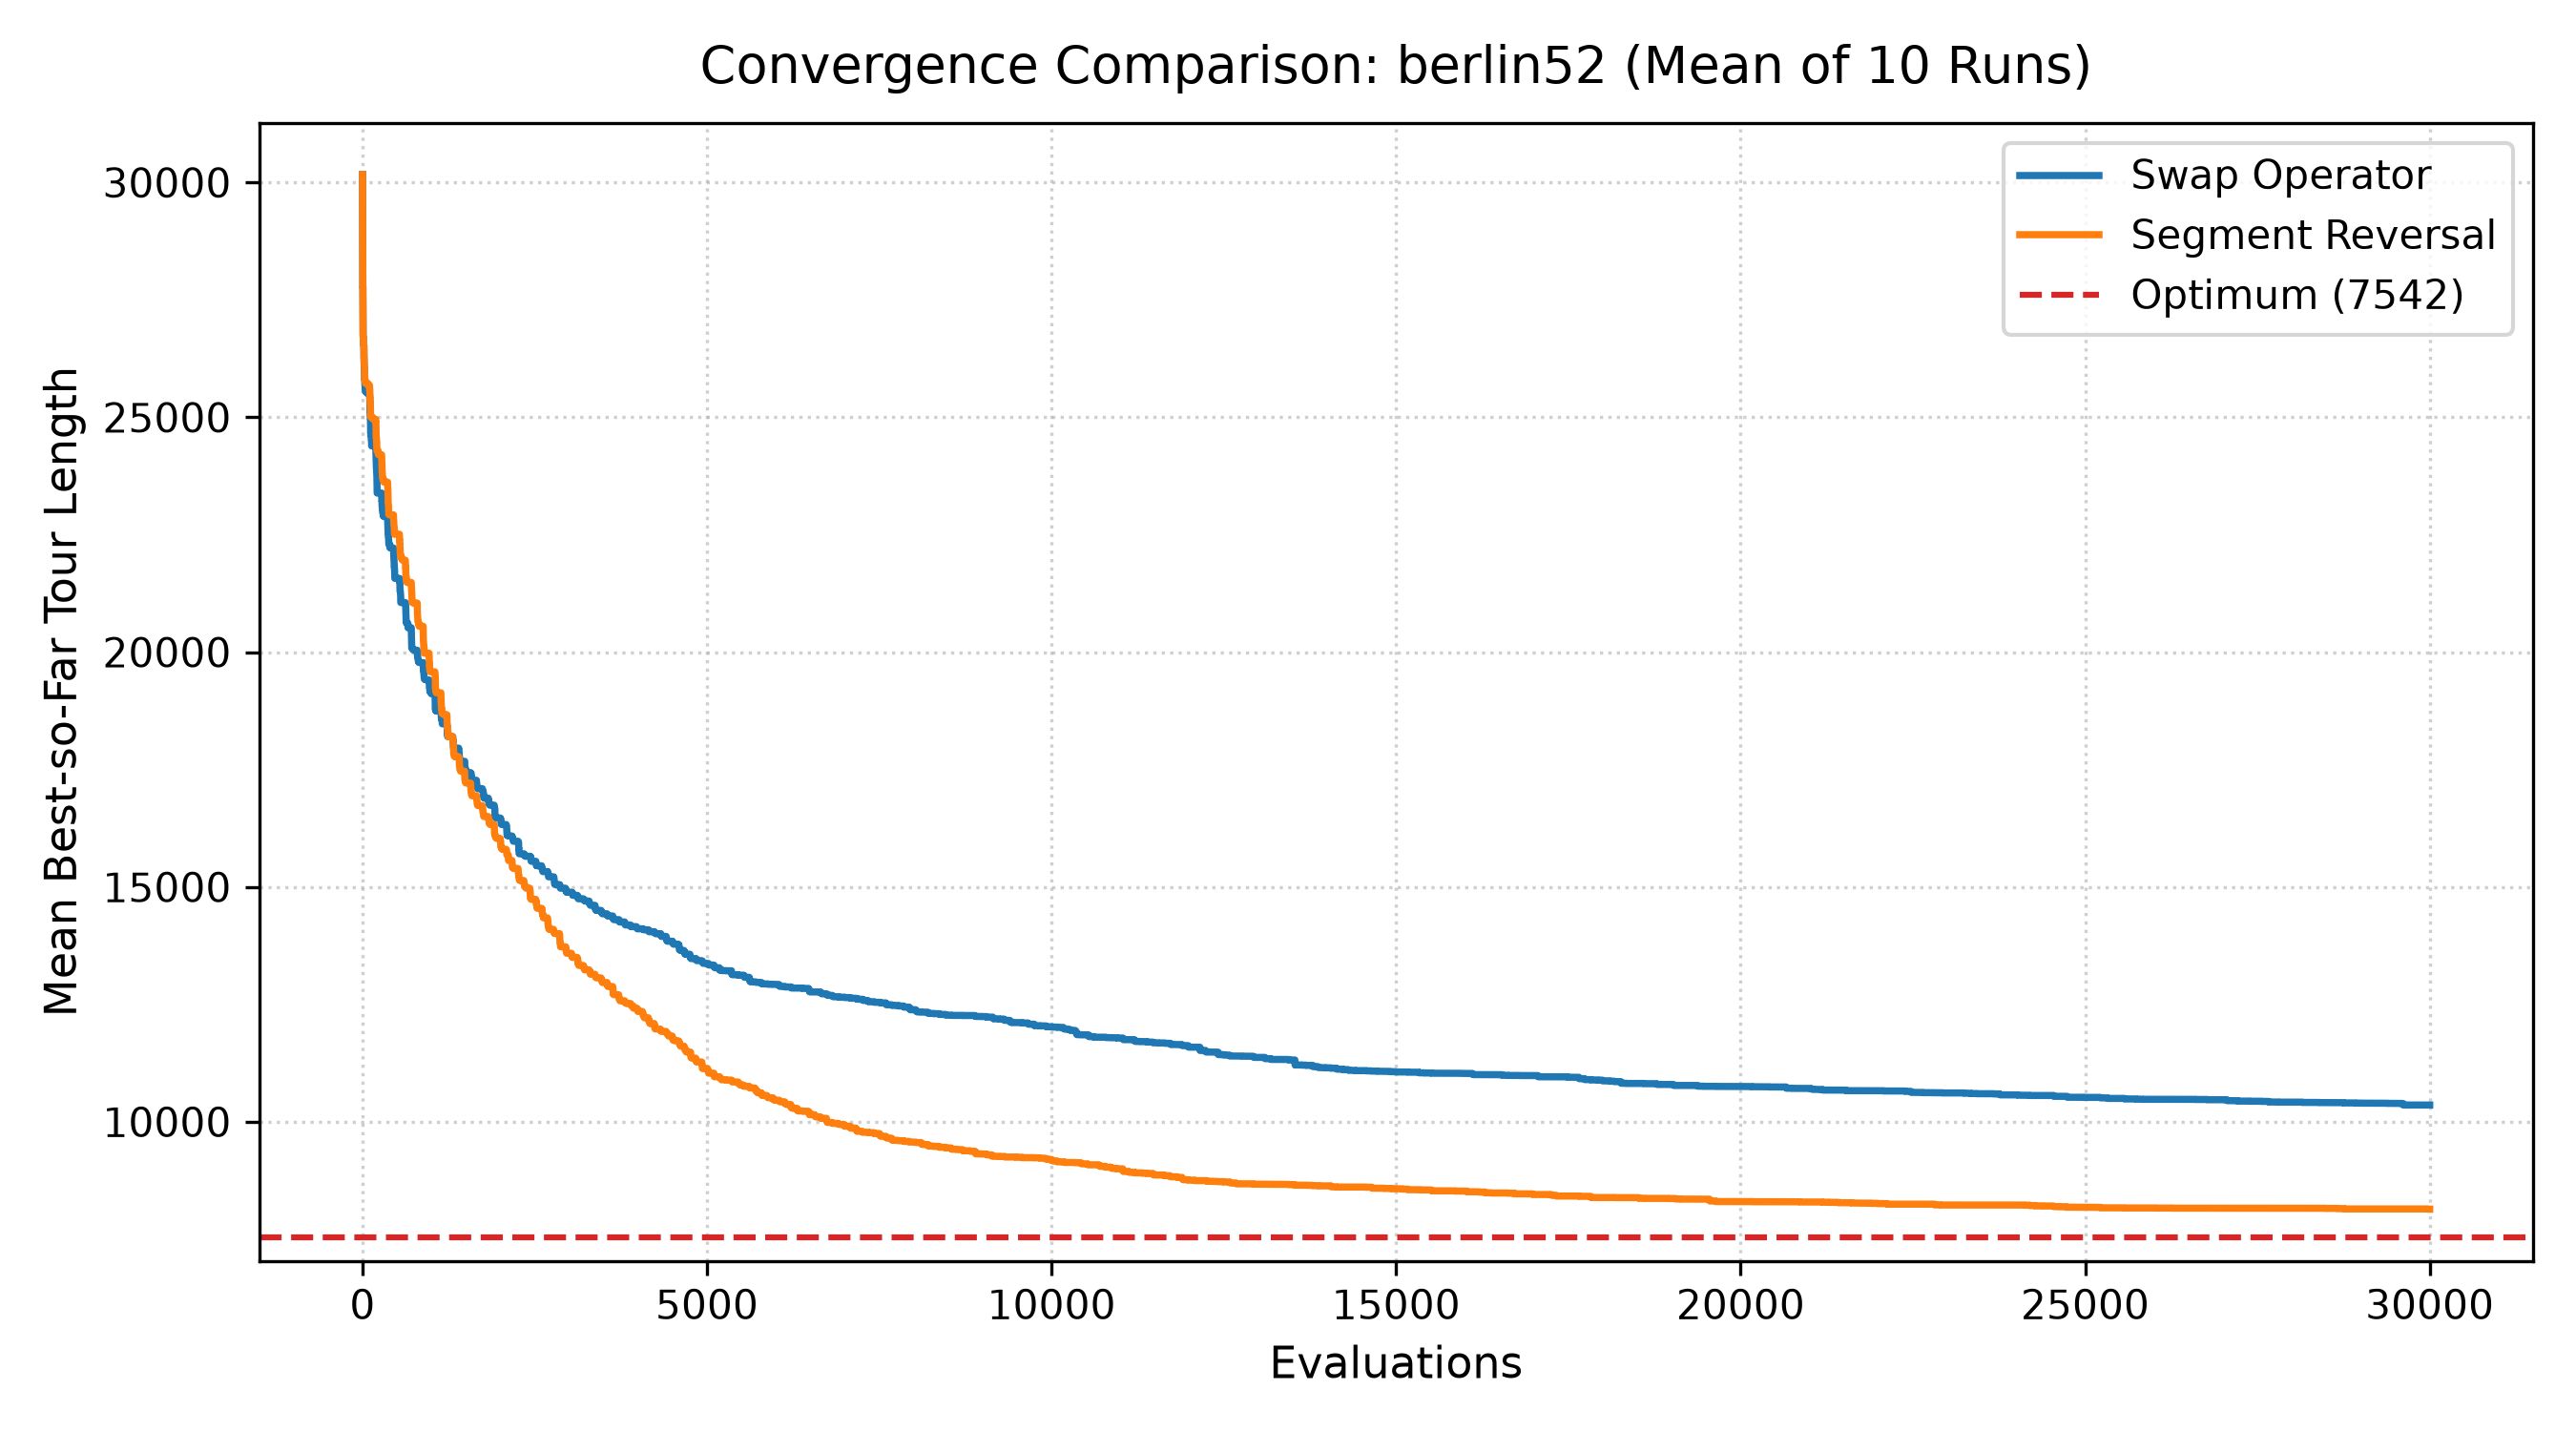
\includegraphics[width=0.85\textwidth]{results/convergence_berlin52.png}
\caption{Mean Best-So-Far Route Length Convergence Across 10 Runs on \texttt{berlin52}}
\label{fig:convergence_berlin52}
\end{figure}

\begin{figure}[htbp]
\centering
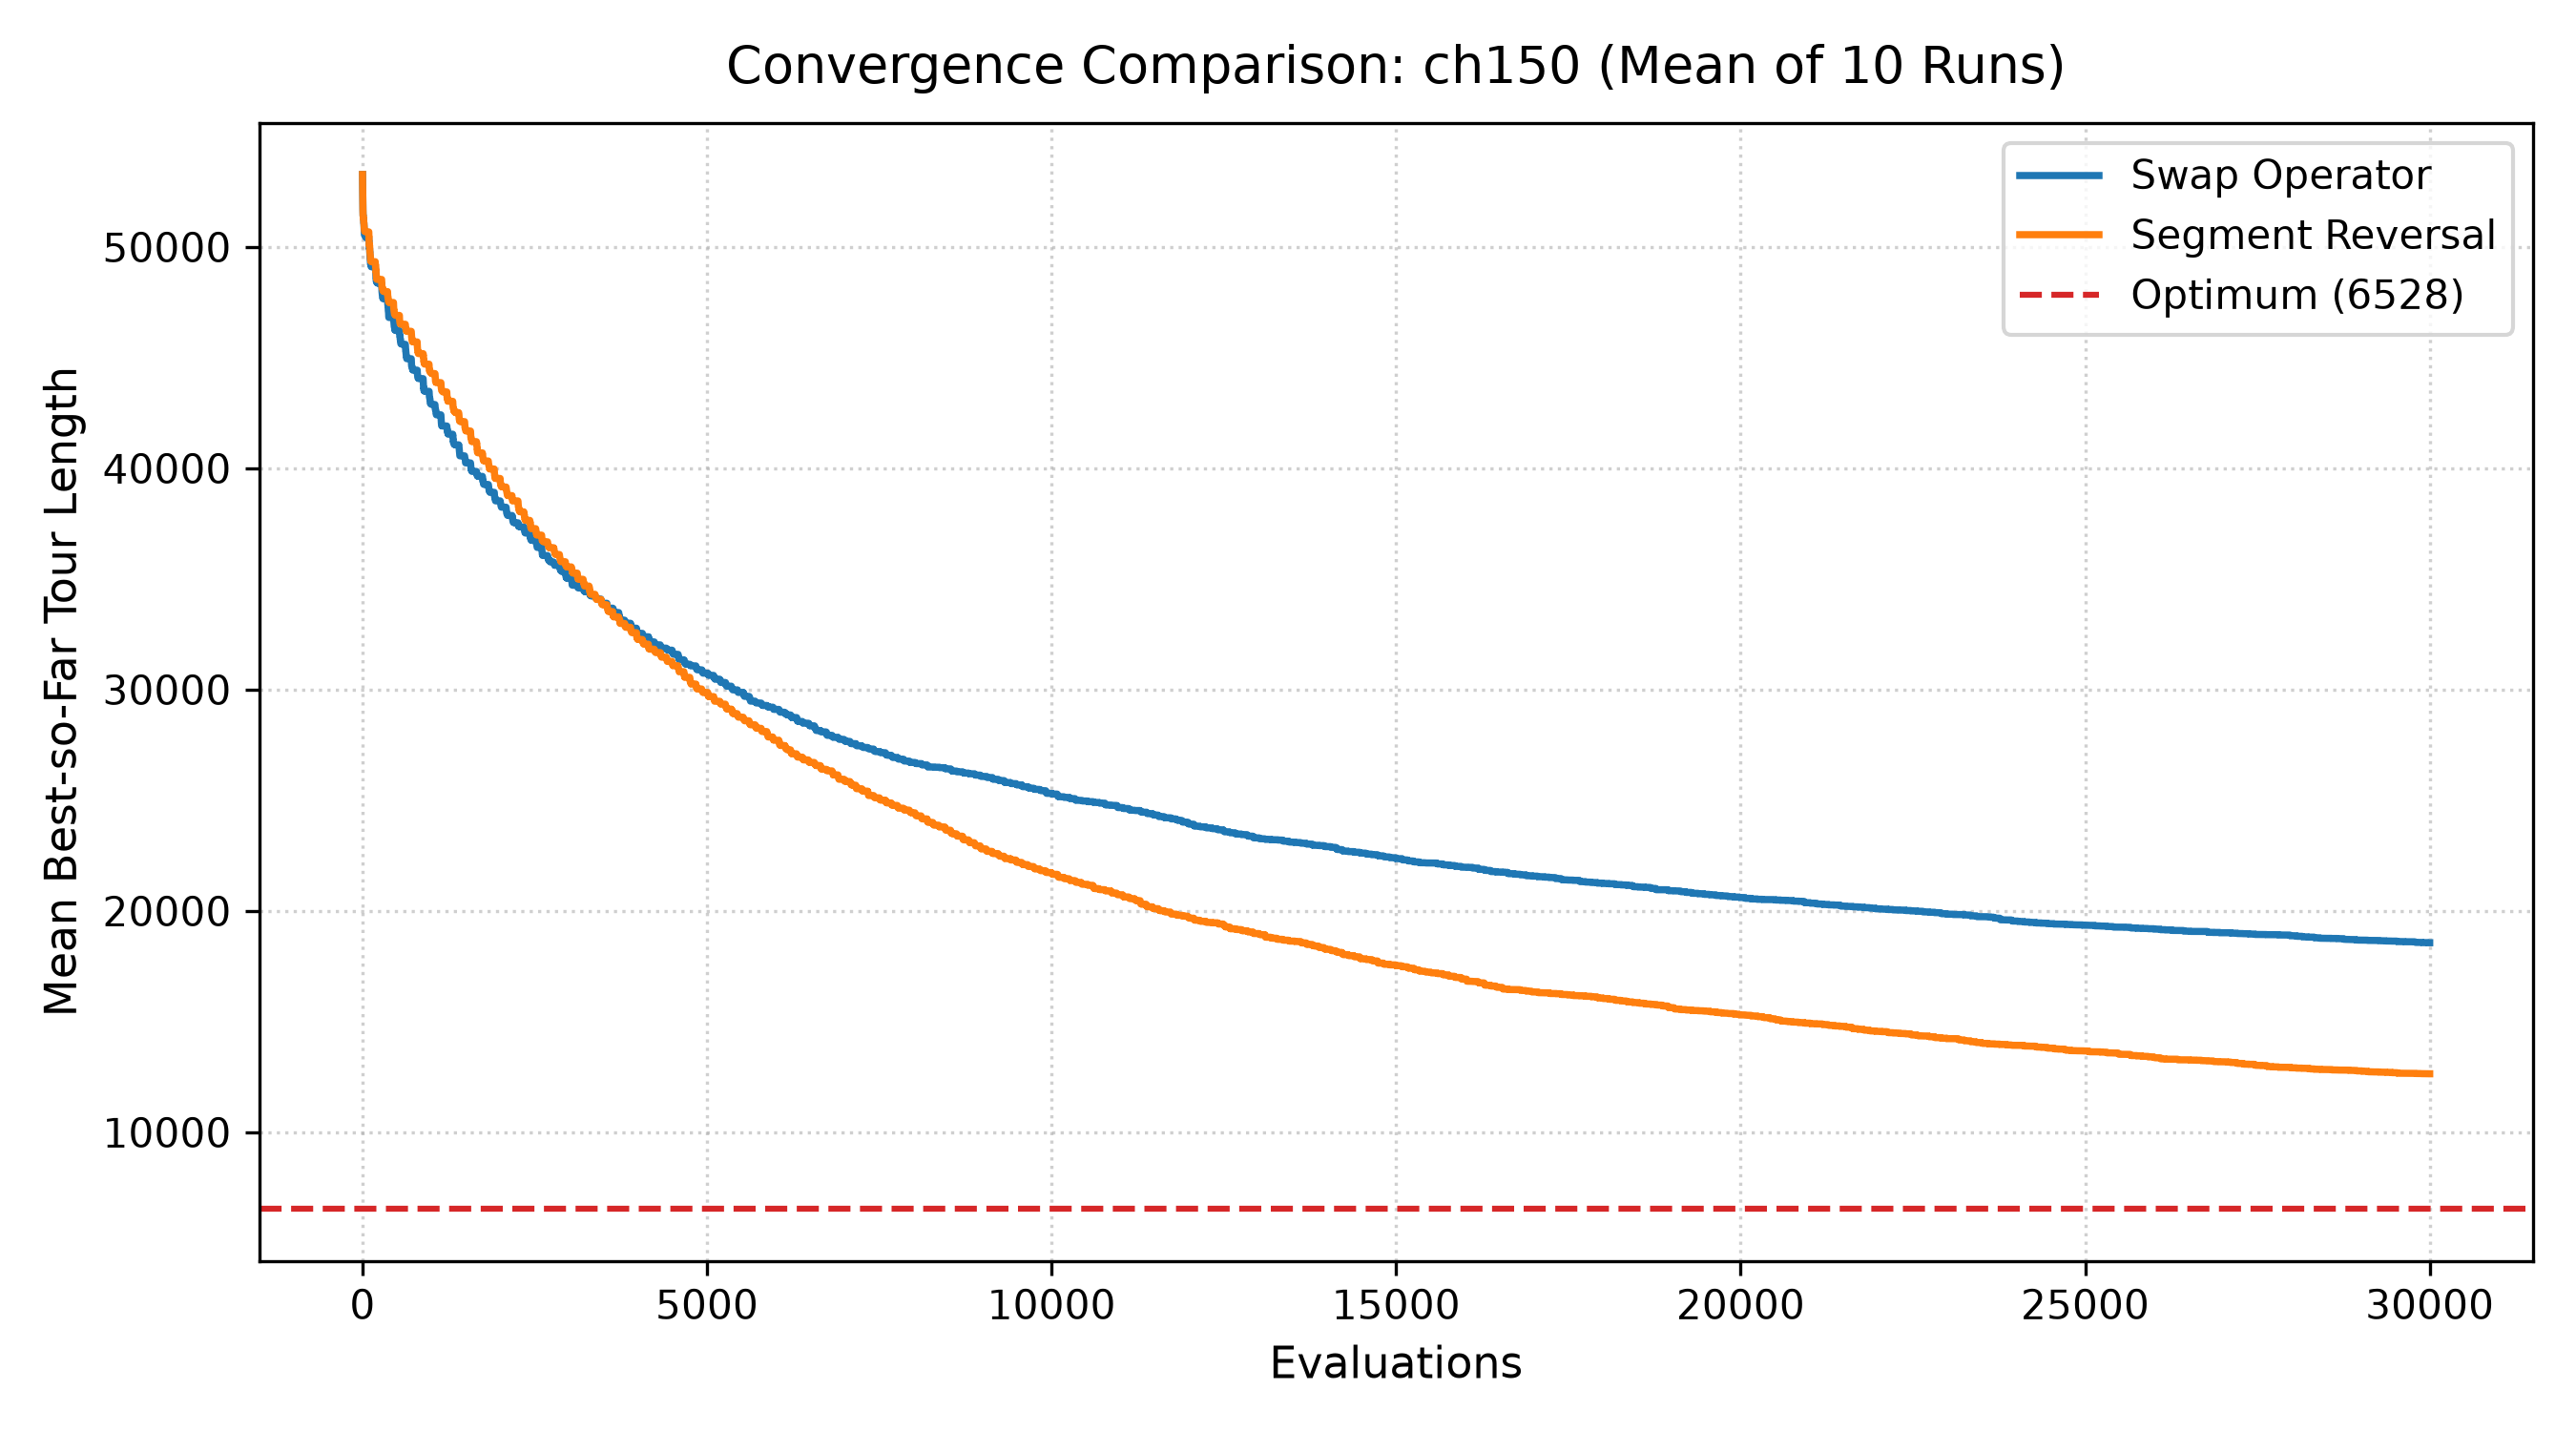
\includegraphics[width=0.85\textwidth]{results/convergence_ch150.png}
\caption{Mean Best-So-Far Route Length Convergence Across 10 Runs on \texttt{ch150}}
\label{fig:convergence_ch150}
\end{figure}

Across all 20 runs on \texttt{berlin52}, the single shortest route was found using the segment reversal operator with seed~8.
This route has a total length of 7,874, which gives a percentage gap of 4.40\% above the known optimum of 7,542.
Figure~\ref{fig:best_route_berlin52} shows this closed route with City~1 marked as the starting depot and the return leg drawn back to the start.
The path follows a clean outer loop without crossing over itself.

\begin{figure}[H]
\centering
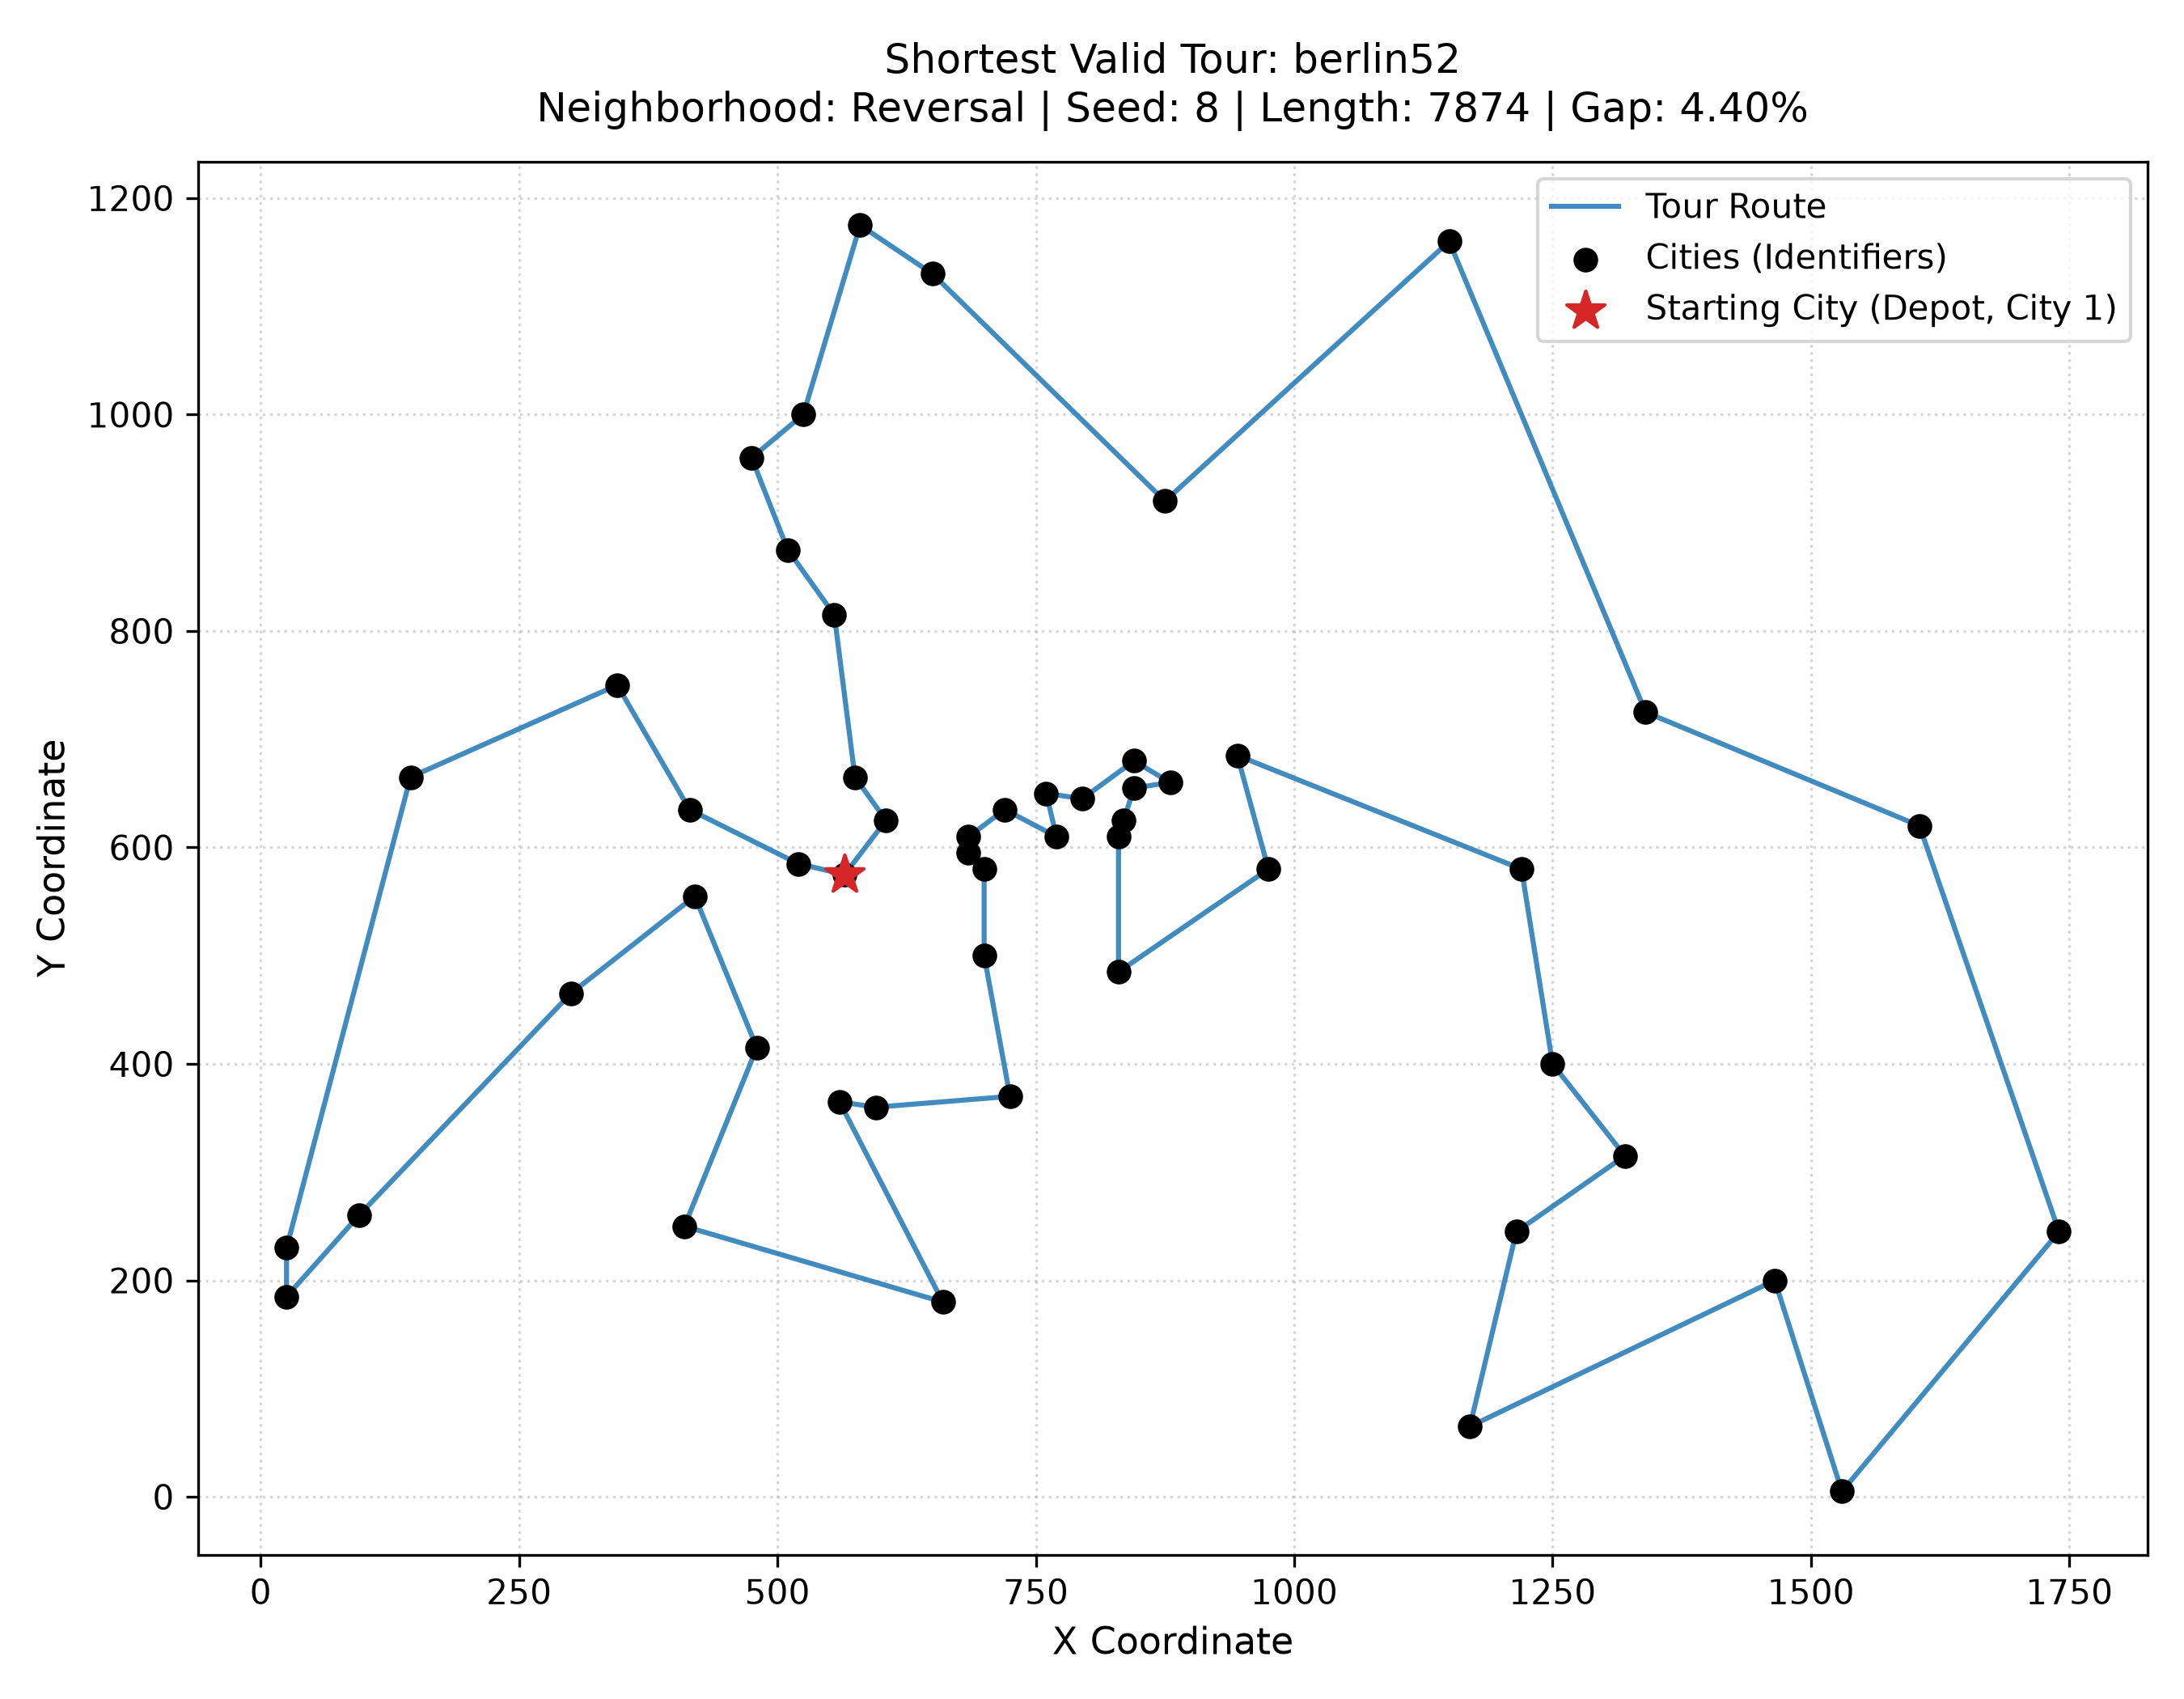
\includegraphics[width=0.8\textwidth]{results/best_route_berlin52.png}
\caption{Shortest Route Discovered on \texttt{berlin52} (\(L = 7{,}874\), Gap \(= 4.40\%\), Reversal Operator, Seed 8)}
\label{fig:best_route_berlin52}
\end{figure}

\subsubsection{Discussion}
The main reason segment reversal outperforms swap comes from how many city connections each move changes during the mutation.
Because the swap operator exchanges two single cities, it breaks up to four connections at once and replaces them with new ones, which can often lead to the destruction of good partial routes that were already found.
The segment reversal operator only breaks two connections at the ends of the chosen segment and keeps all inner connections intact in reverse order.
In 2D Euclidean space, an optimal route never crosses itself.
Reversing the segment between two crossing lines directly uncrosses them, where swapping the two single cities cannot untangle crossings as easily without disturbing other parts of the route.

Looking at the convergence over time, both operators make fast progress during the first 2,000 to 5,000 evaluations because almost any local improvement removes the long random jumps in the initial routes.
However, the swap operator runs into stagnation around 8,000 to 10,000 evaluations because single swaps can easily get trapped in local optima and cannot untangle larger parts of the route.
Segment reversal avoids this early stagnation and continues finding steady improvements throughout the full 30,000-evaluation budget.

None of the 120 runs reached the exact TSPLIB optimum and the larger instances highlight the limits of the fixed budget, but with segment reversal, the mean gap stays below 8\% on \texttt{eil51} and \texttt{berlin52} and below 15\% on \texttt{st70} and \texttt{eil76}.
However, as the number of cities grows to 100 and 150, the number of possible routes grows enormously, so 30,000 evaluations only sample a tiny fraction of the search space.
As a result, even segment reversal ends with mean gaps of 41.94\% on \texttt{kroA100} and 93.69\% on \texttt{ch150}, while swap can be considered unsuccessful on these larger instances with gaps of 137.77\% and 184.40\%.

Finally, segment reversal is much more consistent from run to run than swap.
Across all six instances, it achieves lower standard deviations, such as \(SD = 9.97\) versus \(20.16\) on \texttt{eil51} and \(SD = 208.44\) versus \(501.44\) on \texttt{berlin52}.
Combining local search on elite sites with continuous random scouting helps the algorithm converge reliably across different random seeds when paired with a neighborhood move that keeps good route structure.

% References
\printbibliography

\end{document}
